% Park Ranger Quiz: America's National Parks
% Compile with: latexmk -pdf national_parks.tex
\documentclass[aspectratio=169,11pt]{beamer}

\usepackage[T1]{fontenc}
\usepackage{lmodern}
\usepackage{booktabs}
\usepackage{array}
\usepackage{tikz}
\usetikzlibrary{shapes.geometric,positioning,calc,arrows.meta}
\usepackage{pgfplots}
\pgfplotsset{compat=1.18}
\usepackage[most]{tcolorbox}
\graphicspath{{images/}}

% ---------- Colors ----------
\definecolor{navy}{HTML}{1C2541}
\definecolor{oldred}{HTML}{B22234}   % US flag red, also the accent color
\definecolor{oldblue}{HTML}{3C3B6E}  % US flag blue
\definecolor{ink}{HTML}{2B2B2B}
\definecolor{muted}{HTML}{8A8F98}
\definecolor{paper}{HTML}{FFFFFF}
\definecolor{dem}{HTML}{2E5FA3}      % Democrats
\definecolor{rep}{HTML}{C0392B}      % Republicans
\definecolor{austria}{HTML}{C8102E}  % Austria red, for USA-vs-Austria comparisons

% ---------- Minimal theme ----------
\setbeamertemplate{navigation symbols}{}
\setbeamercolor{normal text}{fg=ink, bg=paper}
\setbeamercolor{structure}{fg=navy}
\setbeamercolor{frametitle}{fg=navy}
\setbeamercolor{alerted text}{fg=oldred}
\setbeamercolor{footnote}{fg=muted}
\setbeamerfont{frametitle}{size=\Large, series=\bfseries}
\setbeamertemplate{itemize item}{\color{oldred}\textbullet}
\setbeamertemplate{itemize subitem}{\color{muted}--}
\setbeamertemplate{enumerate item}{\color{oldred}\insertenumlabel.}
\setbeamersize{text margin left=1.1cm, text margin right=1.1cm}
\hypersetup{colorlinks=true, urlcolor=dem, linkcolor=navy}

\setbeamertemplate{frametitle}{%
  \vspace*{0.5cm}%
  \usebeamerfont{frametitle}\usebeamercolor[fg]{frametitle}\insertframetitle\par
  \vspace{0.15cm}{\color{navy!15}\rule{\textwidth}{0.4pt}}\par}

\setbeamertemplate{footline}{%
  \hfill{\tiny\color{muted}\insertframenumber}\hspace*{0.6cm}\vspace*{0.35cm}}


% "Think" question slides: \begin{thinkframe} ... \end{thinkframe}
\newenvironment{thinkframe}{%
  \begin{frame}[plain,noframenumbering,environment=thinkframe]\centering\Large}{\end{frame}}

% ---------- Helpers ----------
% Small grey source line at the bottom of a frame
\newcommand{\source}[1]{%
  \begin{tikzpicture}[remember picture,overlay]
    \node[anchor=south west, font=\tiny, text=muted, text width=0.85\paperwidth, align=left]
      at ($(current page.south west)+(0.6cm,0.25cm)$) {#1};
  \end{tikzpicture}}

% Quote box with a thin red rule on the left; optional arg e.g. [fontupper=\itshape\small]
\newtcolorbox{textquote}[1][]{%
  enhanced, frame hidden, boxrule=0pt, sharp corners,
  colback=navy!4, borderline west={2pt}{0pt}{oldred},
  left=10pt, right=8pt, top=6pt, bottom=6pt, fontupper=\itshape, #1}

% Photo + name + short bio (use inside a column): \candidate{file}{Name}{bio}
\newcommand{\candidate}[3]{%
  \begin{minipage}[t]{\linewidth}\centering
    \includegraphics[height=3.5cm]{#1}\\[0.5em]
    {\large\bfseries\color{navy}#2}\\[0.4em]
    \begin{minipage}{0.9\linewidth}\raggedright\small #3\end{minipage}
  \end{minipage}}

% Big number with a caption (use inside a column): \bignum{color}{91\%}{caption}
\newcommand{\bignum}[3]{%
  \begin{minipage}[t]{\linewidth}\centering
    {\fontsize{34}{38}\selectfont\bfseries\color{#1}#2}\\[0.3em]
    {\small #3}
  \end{minipage}}

% US flag drawn in TikZ (hoist height = #1), e.g. \usflag{3cm}
\newcommand{\usflag}[1]{%
  \begin{tikzpicture}[x=#1, y=#1]
    \def\fly{1.9}
    \foreach \i in {0,...,12} {
      \pgfmathsetmacro{\c}{mod(\i,2)==0 ? 1 : 0}
      \ifdim\c pt=1pt
        \fill[oldred] (0,{1-(\i+1)/13}) rectangle (\fly,{1-\i/13});
      \else
        \fill[white] (0,{1-(\i+1)/13}) rectangle (\fly,{1-\i/13});
      \fi
    }
    \def\cw{0.76} \def\ch{0.5385}
    \fill[oldblue] (0,{1-\ch}) rectangle (\cw,1);
    \foreach \r in {1,...,9} {
      \pgfmathsetmacro{\isodd}{mod(\r,2)}
      \ifdim\isodd pt=1pt
        \foreach \k in {0,...,5}
          \node[star, star points=5, star point ratio=2.618, fill=white, inner sep=0pt,
                minimum size=0.0616*#1] at ({(2*\k+1)*\cw/12},{1-\r*\ch/10}) {};
      \else
        \foreach \k in {0,...,4}
          \node[star, star points=5, star point ratio=2.618, fill=white, inner sep=0pt,
                minimum size=0.0616*#1] at ({(2*\k+2)*\cw/12},{1-\r*\ch/10}) {};
      \fi
    }
    \draw[ink!30, line width=0.3pt] (0,0) rectangle (\fly,1);
  \end{tikzpicture}}

% Agree/disagree spectrum for "spectrum game" activities
\newcommand{\spectrum}{%
  
\begin{tikzpicture}
    \shade[left color=oldblue, right color=oldred, rounded corners=2pt] (0,0) rectangle (11,0.18);
    \node[anchor=north, font=\small, text=oldblue] at (0,-0.15) {Strongly disagree};
    \node[anchor=north, font=\small, text=muted] at (5.5,-0.15) {Neutral};
    \node[anchor=north, font=\small, text=oldred] at (11,-0.15) {Strongly agree};
    \fill[paper, draw=muted] (5.5,0.09) circle (2.5pt);
  \end{tikzpicture}}

% One statement per slide: \statement{number}{total}{text}
\newcommand{\statement}[3]{%
  \begin{frame}[plain]
    \vfill
    \begin{center}
      {\small\color{muted}Statement #1 of #2}\\[1.2em]
      {\LARGE\bfseries #3}
    \end{center}
    \vfill
    \begin{center}\spectrum\end{center}
    \vspace{1.2cm}
  \end{frame}}


% ---------- Quiz helpers ----------
\newcommand{\credit}[1]{\\[0.2em]{\tiny\color{muted}#1\par}}

% Dots on the US map (coordinates = pixels of the 1280x792 map image)
\newcommand{\mapdot}[3]{%
  \node[circle, fill=navy, text=white, font=\scriptsize\bfseries, inner sep=0pt, minimum size=0.42cm] at (#1,#2) {#3};}
\newcommand{\hitdot}[3]{%
  \only<1>{\node[circle, fill=navy, text=white, font=\scriptsize\bfseries, inner sep=0pt, minimum size=0.42cm] at (#1,#2) {#3};}%
  \only<2>{\node[circle, fill=oldred, draw=white, line width=1pt, text=white, font=\small\bfseries, inner sep=0pt, minimum size=0.6cm] at (#1,#2) {#3};}}

% "Where is this?" slide: \whereis{Round 1}{photo}{credit}{map file}{map px width}{dots}{answer}
\newcommand{\whereis}[7]{%
  \begin{frame}[plain]
    \begin{tikzpicture}[remember picture,overlay]
      \begin{scope}
        \clip (current page.north west) rectangle ($(current page.south west)+(9.7cm,0)$);
        \node[inner sep=0pt] at ($(current page.west)+(4.85cm,0)$) {\includegraphics[height=\paperheight]{#2}};
      \end{scope}
      \node[anchor=south west, font=\tiny, text=white, inner sep=2pt, fill=black, fill opacity=0.45, text opacity=1]
        at ($(current page.south west)+(0.15cm,0.15cm)$) {#3};
      \node[anchor=north west, font=\small\bfseries, text=oldred] at ($(current page.north west)+(10.1cm,-0.75cm)$) {\MakeUppercase{#1}};
      \node[anchor=north west, font=\LARGE\bfseries, text=navy] at ($(current page.north west)+(10.1cm,-1.25cm)$) {Where is this?};
      \begin{scope}[shift={($(current page.north west)+(10.2cm,-2.6cm)$)}, x={(5.4cm/#5,0)}, y={(0,-5.4cm/#5)}]
        \node[anchor=north west, inner sep=0pt] at (0,0) {\includegraphics[width=5.4cm]{#4}};
        #6
      \end{scope}
      \only<2>{\node[anchor=north west, text width=5.5cm, align=left, font=\large] at ($(current page.north west)+(10.1cm,-6.5cm)$) {#7};}
    \end{tikzpicture}
  \end{frame}}

% Answer options A-D
\newcommand{\opt}[2]{{\bfseries\color{navy}#1}\quad #2}

\begin{document}

% ---------- Title slide ----------
\begin{frame}[plain]
  \begin{columns}[c]
    \begin{column}{0.47\textwidth}
      {\fontsize{30}{34}\selectfont\bfseries\color{navy} Park Ranger\\Quiz}\\[0.8em]
      {\Large\color{muted} America's national parks}\\[0.6em]
      {\color{oldred}\rule{3cm}{1.5pt}}
    \end{column}
    \begin{column}{0.5\textwidth}
      \centering
      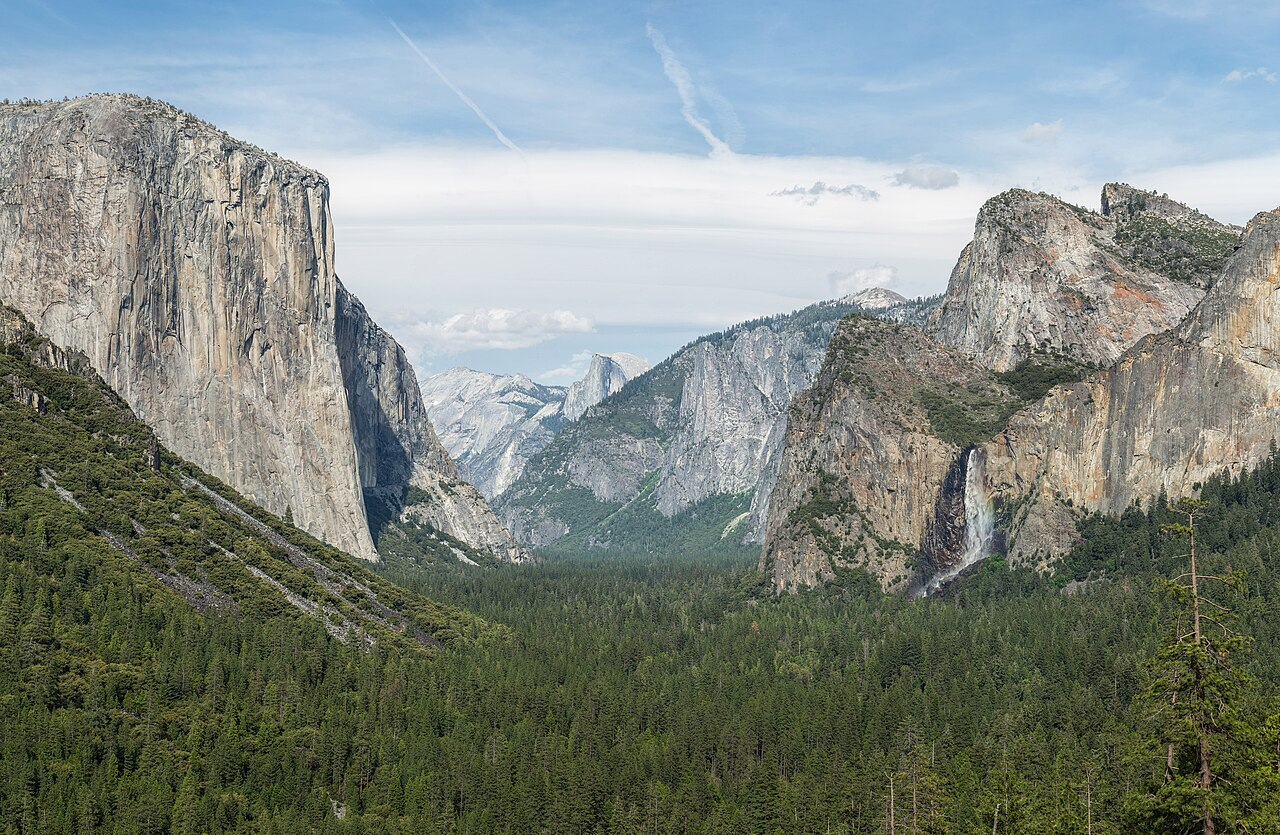
\includegraphics[width=\linewidth]{tunnelview.jpg}
      \credit{Yosemite Valley. Photo: Diliff, CC BY-SA 3.0}
    \end{column}
  \end{columns}
\end{frame}

\begin{frame}{How to play}
  \begin{columns}[c]
    \begin{column}{0.5\textwidth}
      \begin{itemize}\setlength{\itemsep}{0.8em}
        \item Teams of 3 or 4
        \item \alert{Two guesses} per park
        \item Write your answer, hold it up
        \item Keep your own score
        \item Best team: \alert{head ranger}
      \end{itemize}
    \end{column}
    \begin{column}{0.42\textwidth}
      \centering
      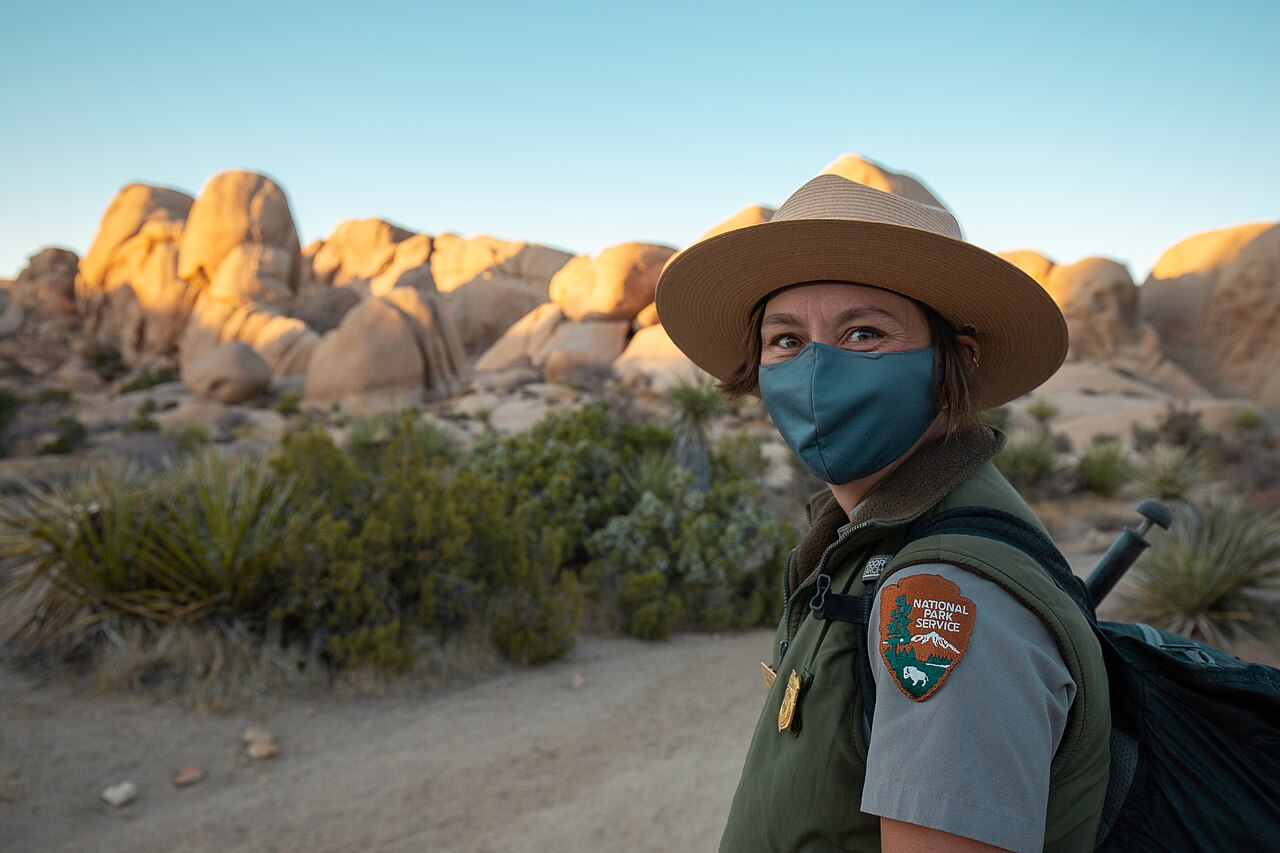
\includegraphics[width=\linewidth]{ranger.jpg}
      \credit{A park ranger. National Park Service, public domain}
    \end{column}
  \end{columns}
\end{frame}

\begin{frame}{National parks}
  \vspace{0.6cm}
  \begin{columns}[T]
    \begin{column}{0.35\textwidth}\bignum{austria}{6}{Austria}\end{column}
    \begin{column}{0.35\textwidth}\bignum{oldblue}{64}{USA}\end{column}
  \end{columns}
  \vspace{1cm}
  \centering{\small\color{muted} The newest: Chiricahua, Arizona (October 2026)\par}
  \source{Source: National Park Service (Oct.\ 2026).}
\end{frame}

\begin{frame}{How big is big?}
  \centering
  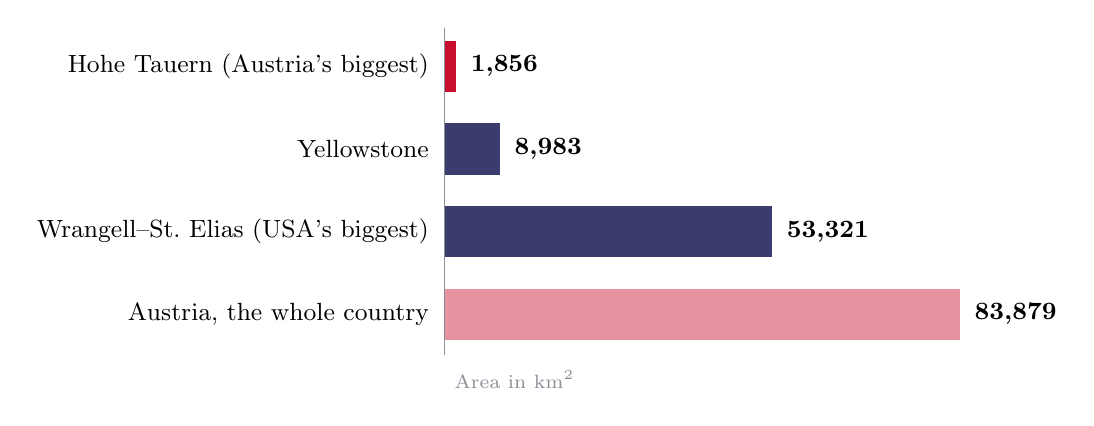
\begin{tikzpicture}[x=0.078cm, y=-1.05cm]   % 1 unit = 1,000 km^2
    \foreach \y/\lab/\val/\txt/\col in {
        0/{Hohe Tauern (Austria's biggest)}/1.856/{1,856}/austria,
        1/{Yellowstone}/8.983/{8,983}/oldblue,
        2/{Wrangell--St.\ Elias (USA's biggest)}/53.321/{53,321}/oldblue,
        3/{Austria, the whole country}/83.879/{83,879}/austria!45} {
      \fill[\col] (0,\y) rectangle (\val,\y+0.62);
      \node[anchor=east, font=\small] at (-1,\y+0.31) {\lab};
      \node[anchor=west, font=\small\bfseries] at (\val+0.8,\y+0.31) {\txt};
    }
    \draw[muted] (0,-0.15) -- (0,3.8);
    \node[font=\scriptsize, text=muted, anchor=west] at (0,4.1) {Area in km$^2$};
  \end{tikzpicture}

  \vspace{0.5em}
  The biggest US park is almost \alert{two thirds of Austria}.
  \source{Sources: National Park Service; Nationalpark Hohe Tauern; Statistik Austria.}
\end{frame}

% ===================== Round 1 =====================
\section{Round 1}
\whereis{Round 1}{prismatic.jpg}{Photo: Jim Peaco, NPS, public domain}{usmap.png}{1280}
  {\hitdot{335}{190}{A}\mapdot{1030}{680}{B}\mapdot{265}{490}{C}\mapdot{1200}{110}{D}}
  {\alert{\textbf{A: Wyoming}}\\[0.2em]{\normalsize Yellowstone National Park}}

\begin{frame}{Yellowstone}
  \begin{columns}[c]
    \begin{column}{0.52\textwidth}
      \begin{itemize}\setlength{\itemsep}{0.9em}
        \item The world's \alert{first} national park (1872)
        \item Sits on a supervolcano
        \item Geyser ``Old Faithful'': every 90 minutes
        \item Bison, wolves, grizzly bears
      \end{itemize}
    \end{column}
    \begin{column}{0.42\textwidth}
      \centering
      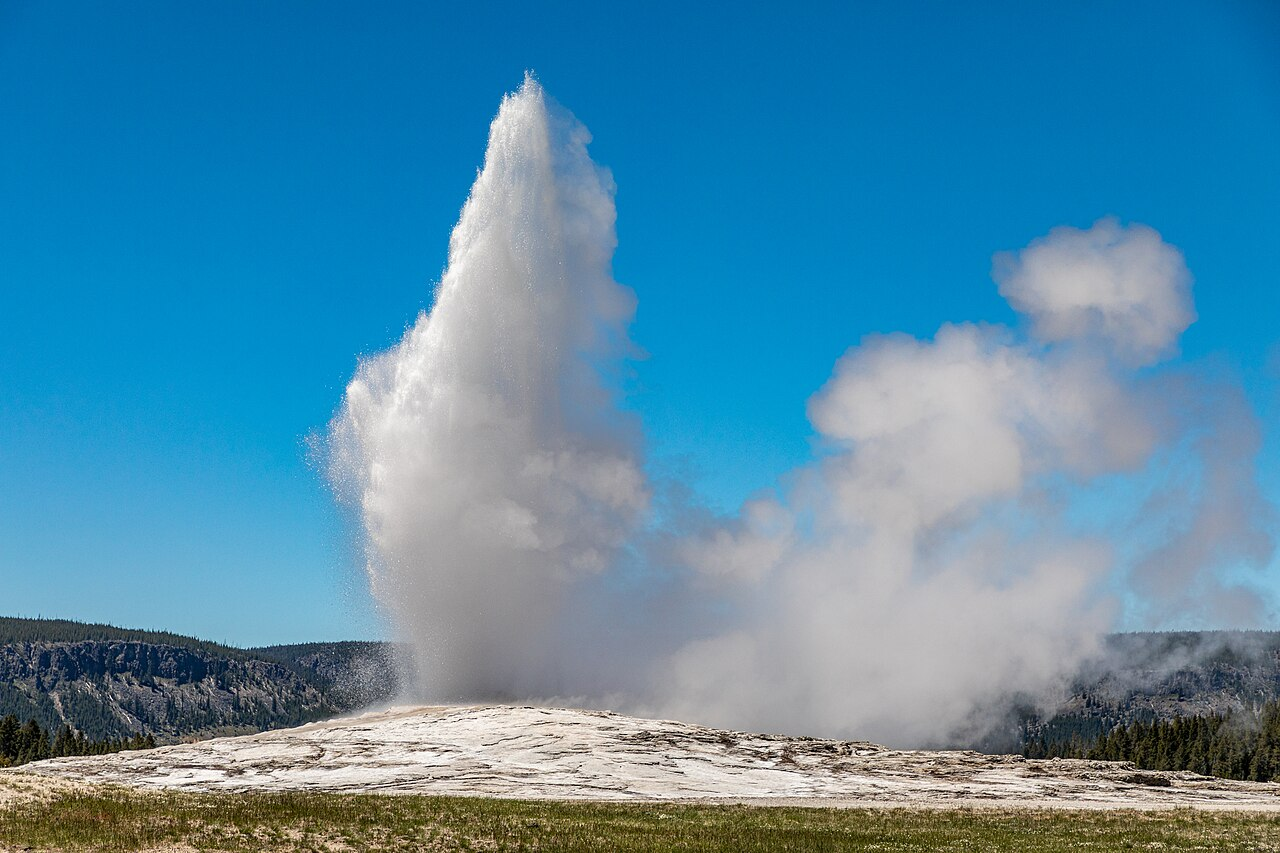
\includegraphics[width=\linewidth]{oldfaithful.jpg}
      \credit{Old Faithful. Photo: Dietmar Rabich, CC BY-SA 4.0}
    \end{column}
  \end{columns}
\end{frame}

\begin{frame}{Guess: the most dangerous animal}
  \begin{columns}[c]
    \begin{column}{0.5\textwidth}
      Which animal injures the \alert{most visitors} in Yellowstone?\\[1em]
      \opt{A}{Grizzly bear}\\[0.45em]
      \opt{B}{Wolf}\\[0.45em]
      \opt{C}{Bison}\\[0.45em]
      \opt{D}{Elk}\\[1em]
      \uncover<2>{\alert{\textbf{C: Bison.}} 900 kg, 55 km/h, and tourists take selfies with them.}
    \end{column}
    \begin{column}{0.44\textwidth}
      \centering
      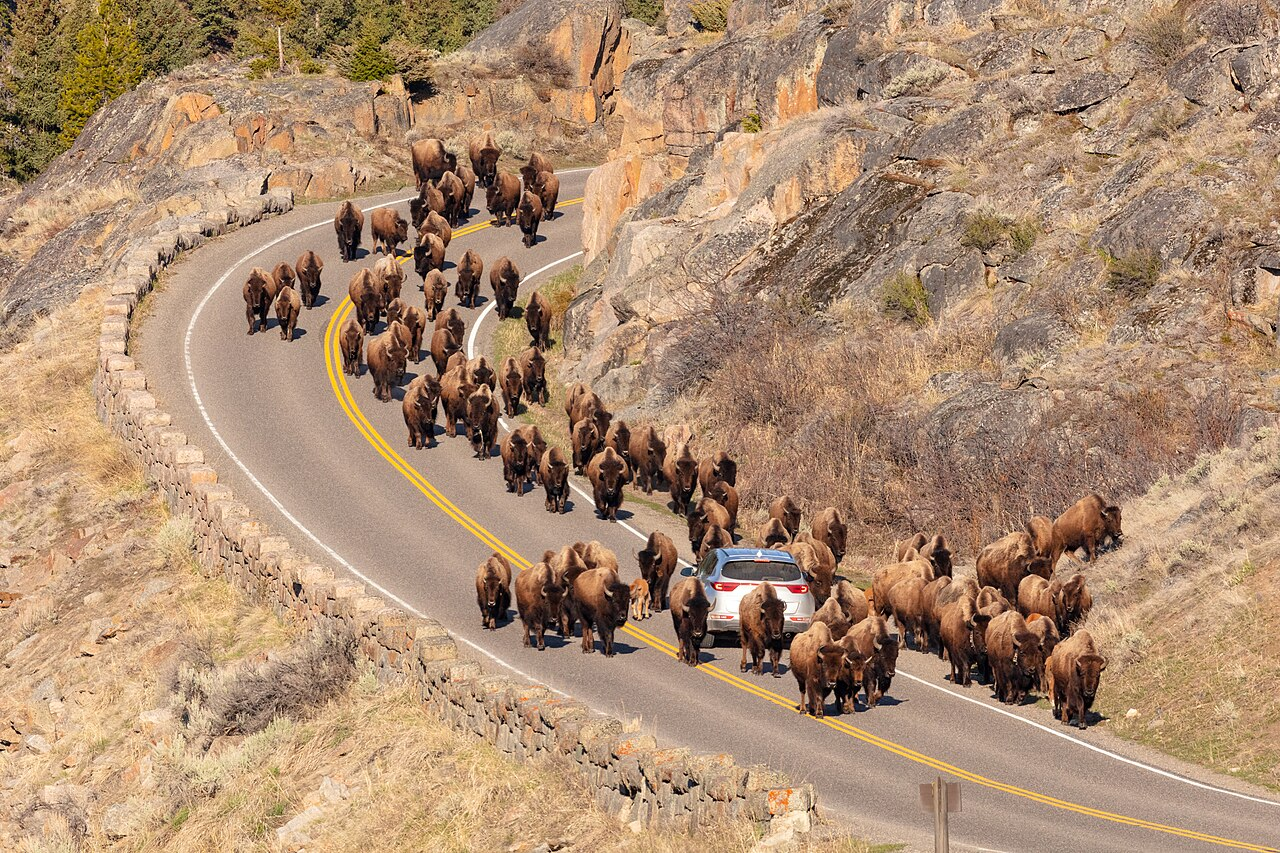
\includegraphics[width=\linewidth]{bison.jpg}
      \credit{Yellowstone National Park, public domain}
    \end{column}
  \end{columns}
  \source{Source: National Park Service.}
\end{frame}

% ===================== Round 2 =====================
\section{Round 2}
\whereis{Round 2}{grandcanyon2.jpg}{Photo: G. Lamar, CC BY 2.0}{usmap.png}{1280}
  {\mapdot{560}{600}{A}\hitdot{255}{430}{B}\mapdot{425}{355}{C}\mapdot{120}{150}{D}}
  {\alert{\textbf{B: Arizona}}\\[0.2em]{\normalsize Grand Canyon National Park}}

\begin{frame}{Grand Canyon}
  \begin{columns}[c]
    \begin{column}{0.52\textwidth}
      \begin{itemize}\setlength{\itemsep}{0.9em}
        \item Carved by the Colorado River
        \item 446 km long
        \item Up to \alert{1.8 km} deep
        \item That is \alert{13 Stephansdoms}, stacked
      \end{itemize}
    \end{column}
    \begin{column}{0.42\textwidth}
      \centering
      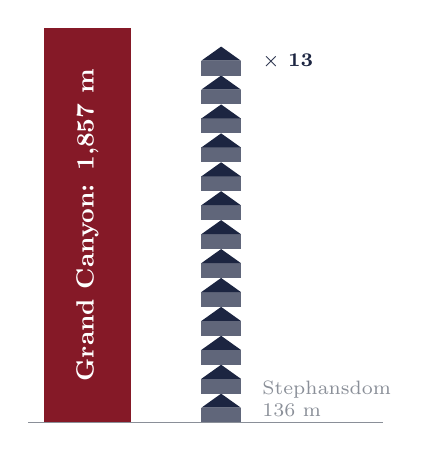
\begin{tikzpicture}[y=0.0027cm, x=1cm]   % 1 unit = 1 m
        % canyon depth
        \fill[oldred!75!black] (0,0) rectangle (1.1,1857);
        \node[font=\small\bfseries, text=white, rotate=90] at (0.55,928) {Grand Canyon: 1,857 m};
        % 13 cathedral towers
        \foreach \i in {0,...,12} {
          \pgfmathsetmacro{\b}{\i*136}
          \pgfmathsetmacro{\m}{\b+70}
          \pgfmathsetmacro{\t}{\b+136}
          \fill[navy!70] (2.0,\b) rectangle (2.5,\m);
          \fill[navy] (2.0,\m) -- (2.5,\m) -- (2.25,\t) -- cycle;
        }
        \draw[muted] (-0.2,0) -- (4.3,0);
        \node[anchor=west, font=\scriptsize, text=muted, align=left] at (2.65,110) {Stephansdom\\136 m};
        \node[anchor=west, font=\scriptsize\bfseries, text=navy] at (2.65,1700) {$\times$ 13};
      \end{tikzpicture}
    \end{column}
  \end{columns}
\end{frame}

\begin{frame}{Guess: deaths}
  \centering
  \vspace{0.6cm}
  {\Large How many people die in the Grand Canyon\\[0.2em] in a typical year?}\\[0.9em]
  {\color{muted} Closest team gets the point.}\\[1.4em]
  \uncover<2>{{\fontsize{34}{38}\selectfont\bfseries\color{oldred} about 12}\\[0.5em]
  More than in any other national park.}
  \source{Source: NPS data for 2010--2020 (134 deaths), via Outforia.}
\end{frame}

% ===================== Round 3 =====================
\section{Round 3}
\whereis{Round 3}{valleyview.jpg}{Photo: King of Hearts, CC BY-SA 3.0}{usmap.png}{1280}
  {\mapdot{150}{60}{A}\mapdot{290}{330}{B}\hitdot{95}{370}{C}\mapdot{150}{650}{D}}
  {\alert{\textbf{C: California}}\\[0.2em]{\normalsize Yosemite National Park}}

\begin{frame}{Yosemite}
  \begin{columns}[c]
    \begin{column}{0.52\textwidth}
      \begin{itemize}\setlength{\itemsep}{0.9em}
        \item Granite cliffs and giant waterfalls
        \item Protected since 1864 (Lincoln)
        \item Giant sequoias: 3,000 years old
        \item ``El Capitan'': a \alert{900 m} wall
      \end{itemize}
    \end{column}
    \begin{column}{0.42\textwidth}
      \centering
      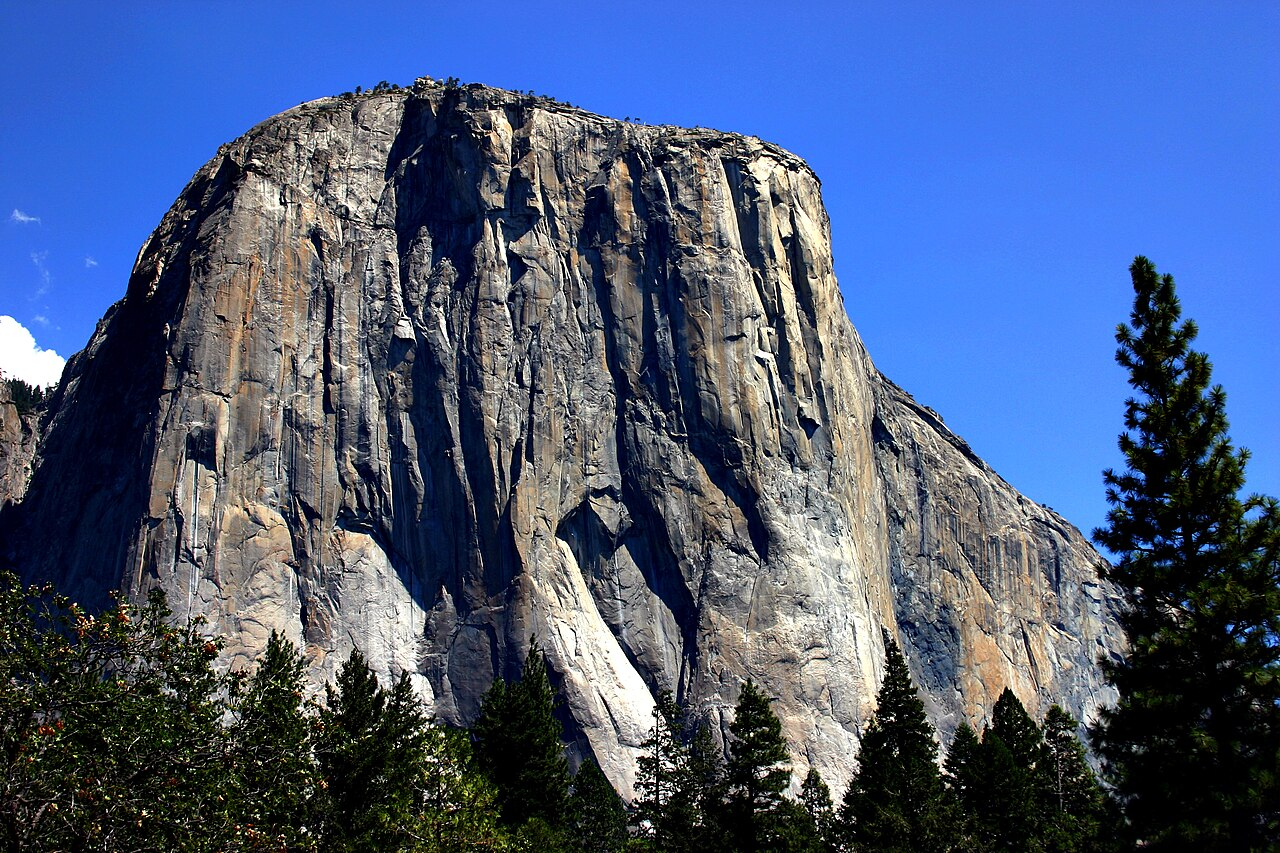
\includegraphics[width=\linewidth]{elcap.jpg}
      \credit{El Capitan. Photo: Mike Murphy, CC BY-SA 3.0}
    \end{column}
  \end{columns}
\end{frame}

\begin{frame}{Guess: no rope}
  \begin{columns}[c]
    \begin{column}{0.5\textwidth}
      2017: Alex Honnold climbs El Capitan \alert{without a rope}.\\[0.8em]
      How long does he need?\\[0.8em]
      {\color{muted} Closest team gets the point.}\\[1.2em]
      \uncover<2>{{\fontsize{22}{26}\selectfont\bfseries\color{oldred}\mbox{3 hours 56 minutes}}}
    \end{column}
    \begin{column}{0.44\textwidth}
      \centering
      \begin{tikzpicture}
        \node[inner sep=0pt] (p) {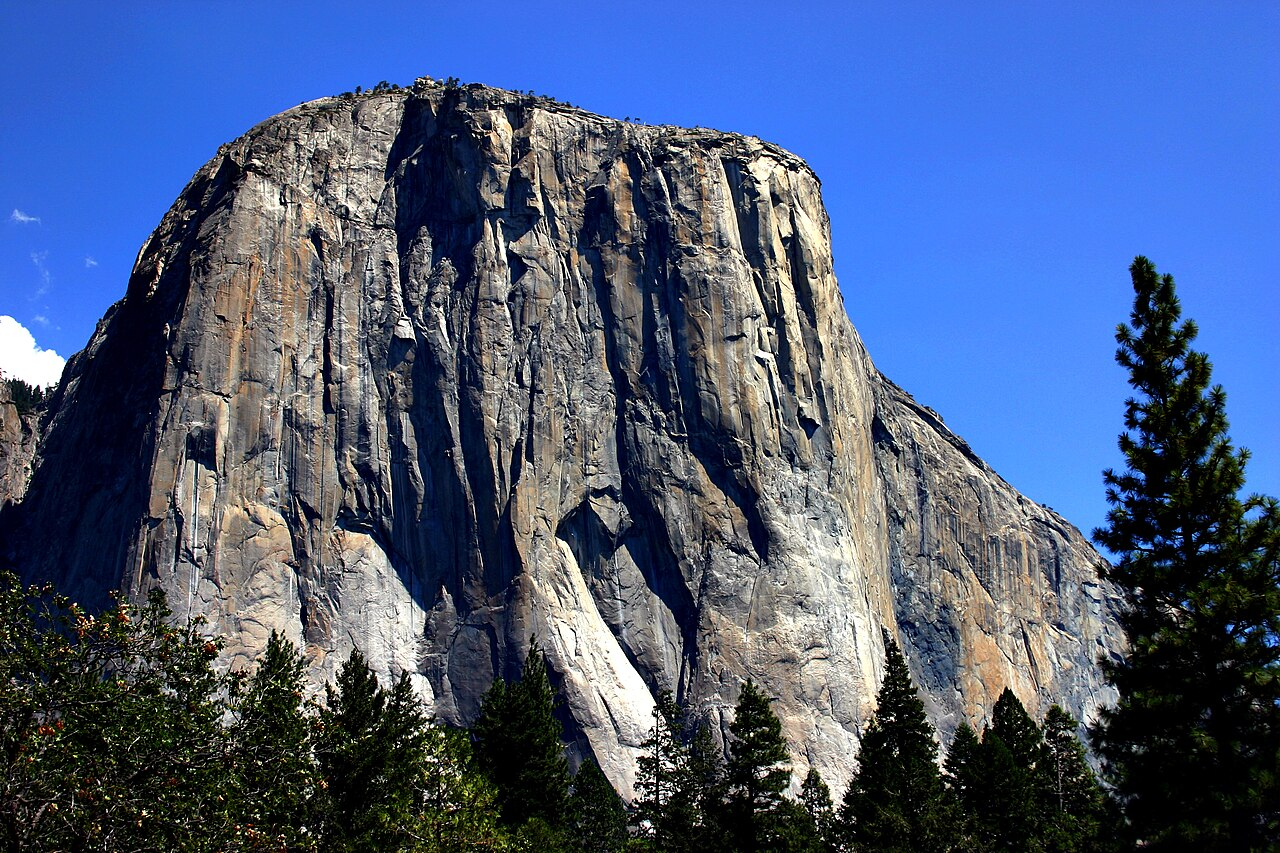
\includegraphics[width=\linewidth]{elcap.jpg}};
        \draw[white, line width=1.2pt, {Latex[length=2mm]}-{Latex[length=2mm]}]
          ($(p.south west)!0.42!(p.south east)+(0,0.75)$) -- ($(p.north west)!0.42!(p.north east)+(0,-0.45)$)
          node[midway, right=2pt, font=\small\bfseries, text=white, fill=black, fill opacity=0.5, text opacity=1, inner sep=2pt] {900 m};
      \end{tikzpicture}
      \credit{Almost 7 Stephansdoms. Photo: Mike Murphy, CC BY-SA 3.0}
    \end{column}
  \end{columns}
\end{frame}

% ===================== Round 4 =====================
\section{Round 4}
\whereis{Round 4}{smokies.jpg}{Photo: USchick, CC BY-SA 3.0}{usmap.png}{1280}
  {\hitdot{955}{440}{A}\mapdot{330}{110}{B}\mapdot{395}{490}{C}\mapdot{680}{140}{D}}
  {\alert{\textbf{A: Tennessee and North Carolina}}\\[0.2em]{\normalsize Great Smoky Mountains National Park}}

\begin{frame}{Guess: the most popular park}
  \begin{columns}[c]
    \begin{column}{0.4\textwidth}
      Which national park gets the \alert{most visitors}?\\[1em]
      \opt{A}{Yellowstone}\\[0.45em]
      \opt{B}{Grand Canyon}\\[0.45em]
      \opt{C}{Yosemite}\\[0.45em]
      \opt{D}{Great Smoky Mountains}
    \end{column}
    \begin{column}{0.56\textwidth}
      \uncover<2>{%
      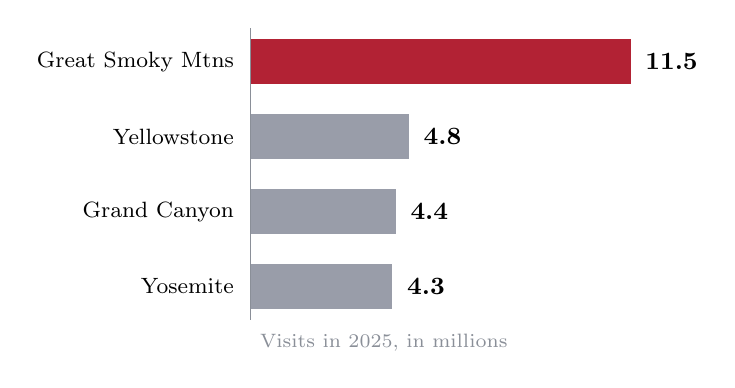
\begin{tikzpicture}[x=0.42cm, y=-0.95cm]   % 1 unit = 1 million visits
        \foreach \y/\lab/\val/\col in {0/Great Smoky Mtns/11.5/oldred, 1/Yellowstone/4.8/navy!45,
                                       2/Grand Canyon/4.4/navy!45, 3/Yosemite/4.3/navy!45} {
          \fill[\col] (0,\y) rectangle (\val,\y+0.6);
          \node[anchor=east, font=\footnotesize] at (-0.2,\y+0.3) {\lab};
          \node[anchor=west, font=\small\bfseries] at (\val+0.15,\y+0.3) {\val};
        }
        \draw[muted] (0,-0.15) -- (0,3.75);
        \node[font=\scriptsize, text=muted, anchor=west] at (0,4.05) {Visits in 2025, in millions};
      \end{tikzpicture}}
    \end{column}
  \end{columns}
  \source{Source: National Park Service (2025 visits, published March 2026).}
\end{frame}

\begin{frame}{Great Smoky Mountains}
  \begin{columns}[c]
    \begin{column}{0.52\textwidth}
      \begin{itemize}\setlength{\itemsep}{0.9em}
        \item \alert{11.5 million} visits a year
        \item More than Austria's whole population
        \item No entrance fee
        \item About 1,900 \alert{black bears}
      \end{itemize}
    \end{column}
    \begin{column}{0.42\textwidth}
      \centering
      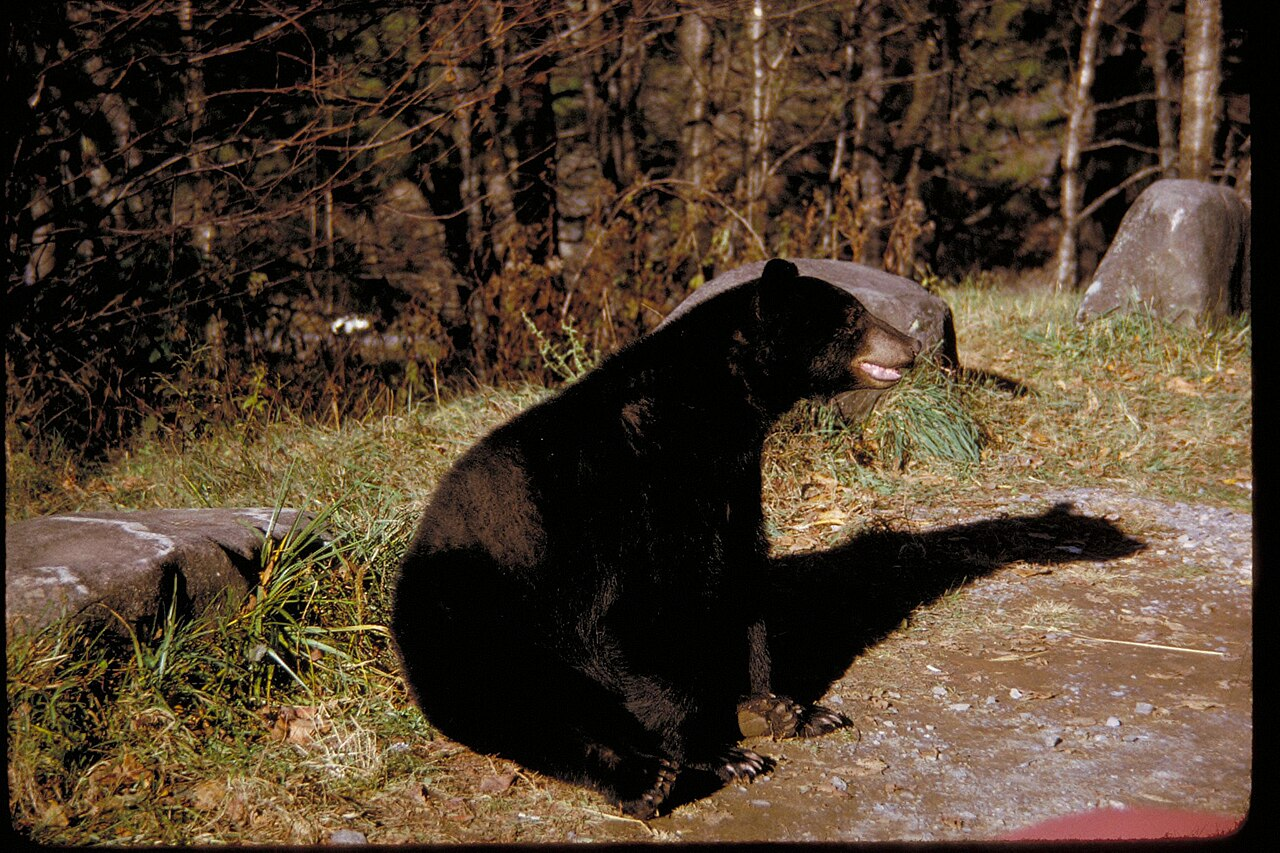
\includegraphics[width=\linewidth]{blackbear.jpg}
      \credit{A black bear in the Smokies. NPS, public domain}
    \end{column}
  \end{columns}
  \source{Source: National Park Service.}
\end{frame}

% ===================== Round 5 =====================
\section{Round 5}
\whereis{Round 5}{mcdonald.jpg}{Photo: TLJones007, CC BY-SA 4.0}{usmap.png}{1280}
  {\mapdot{150}{650}{A}\mapdot{425}{355}{B}\hitdot{270}{80}{C}\mapdot{1127}{165}{D}}
  {\alert{\textbf{C: Montana}}\\[0.2em]{\normalsize Glacier National Park, on the Canadian border}}

\begin{frame}{Guess: what changed?}
  \centering
  \begin{columns}[c]
    \begin{column}{0.3\textwidth}
      \centering
      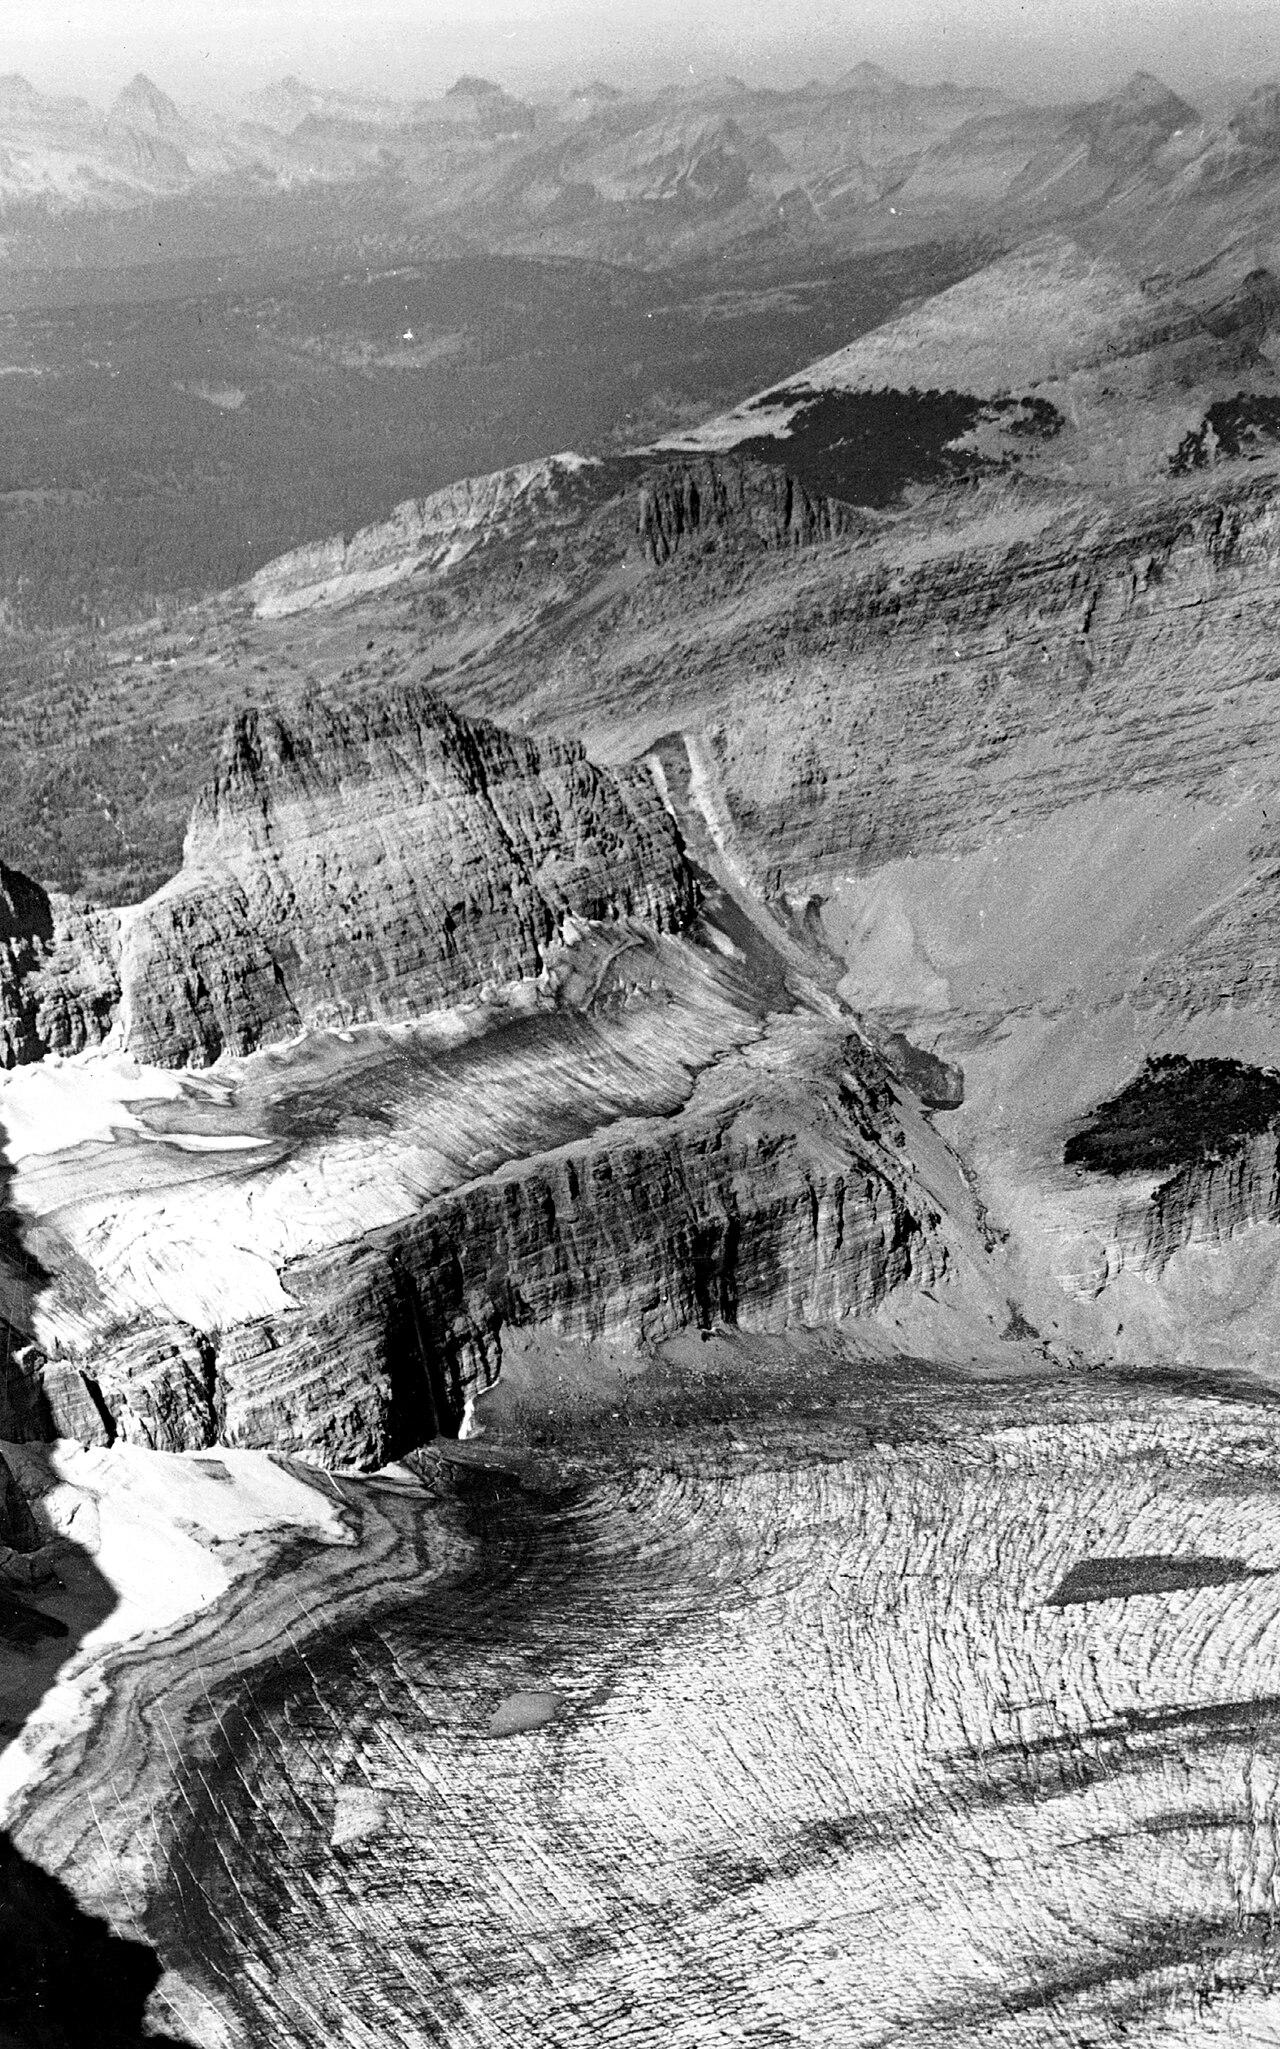
\includegraphics[height=4.1cm]{grinnell1938.jpg}\\[0.2em]
      {\bfseries\color{navy} 1938}
    \end{column}
    \begin{column}{0.5\textwidth}
      \centering
      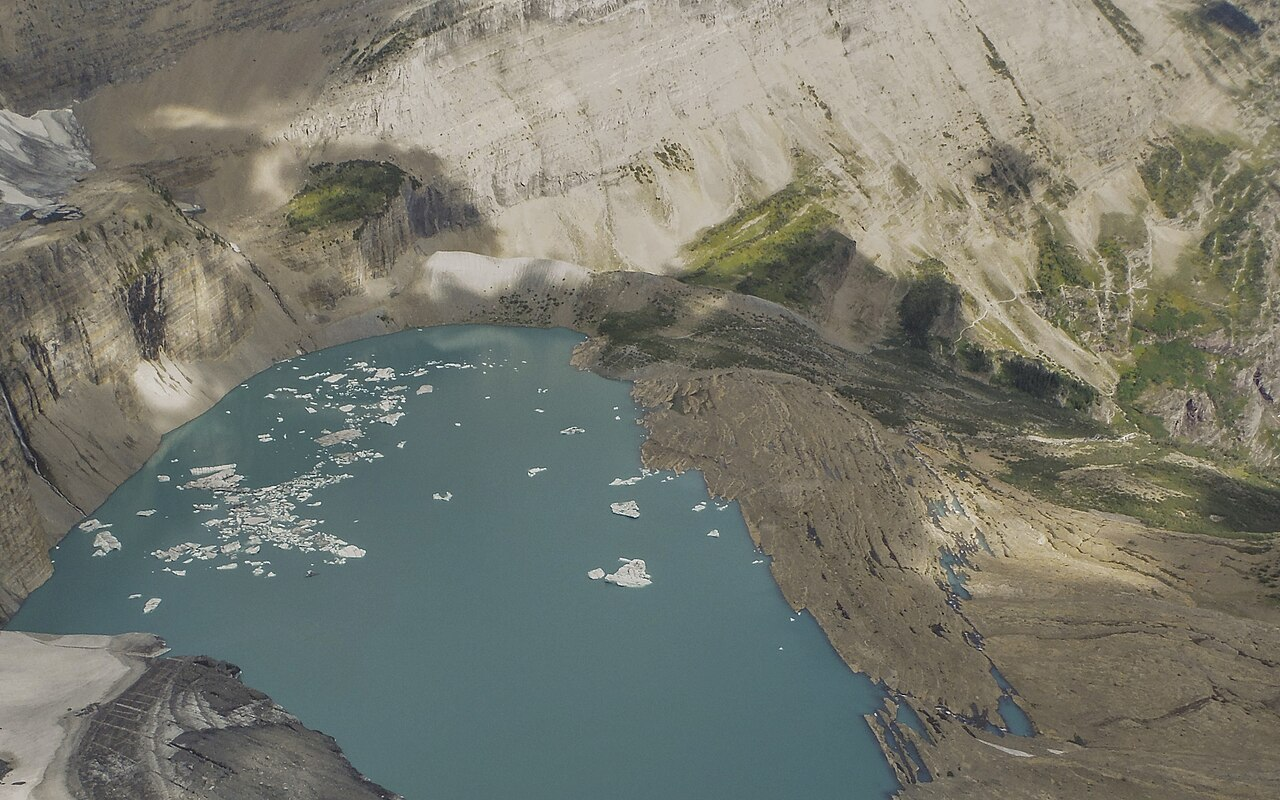
\includegraphics[height=4.1cm]{grinnell2019.jpg}\\[0.2em]
      {\bfseries\color{navy} 2019}
    \end{column}
  \end{columns}
  \vspace{0.9em}
  \only<1>{Same place, 80 years apart. What do you see?}%
  \only<2>{The park's glaciers have shrunk \alert{39\%} on average since 1966.}
  \source{Grinnell Glacier from Mount Gould. Photos: Glacier National Park / USGS, public domain. Figure: USGS (2017).}
\end{frame}

% ===================== Round 6 =====================
\section{Round 6}
\whereis{Round 6}{rushmore2.jpg}{Photo: Dean Franklin, CC BY 2.0}{usmap.png}{1280}
  {\mapdot{985}{398}{A}\hitdot{490}{215}{B}\mapdot{165}{310}{C}\mapdot{1105}{318}{D}}
  {\alert{\textbf{B: South Dakota}}\\[0.2em]{\normalsize Mount Rushmore}}

\begin{frame}{Guess: who are they?}
  \begin{columns}[c]
    \begin{column}{0.52\textwidth}
      \centering
      \begin{tikzpicture}
        \node[inner sep=0pt, anchor=south west] (p) at (0,0) {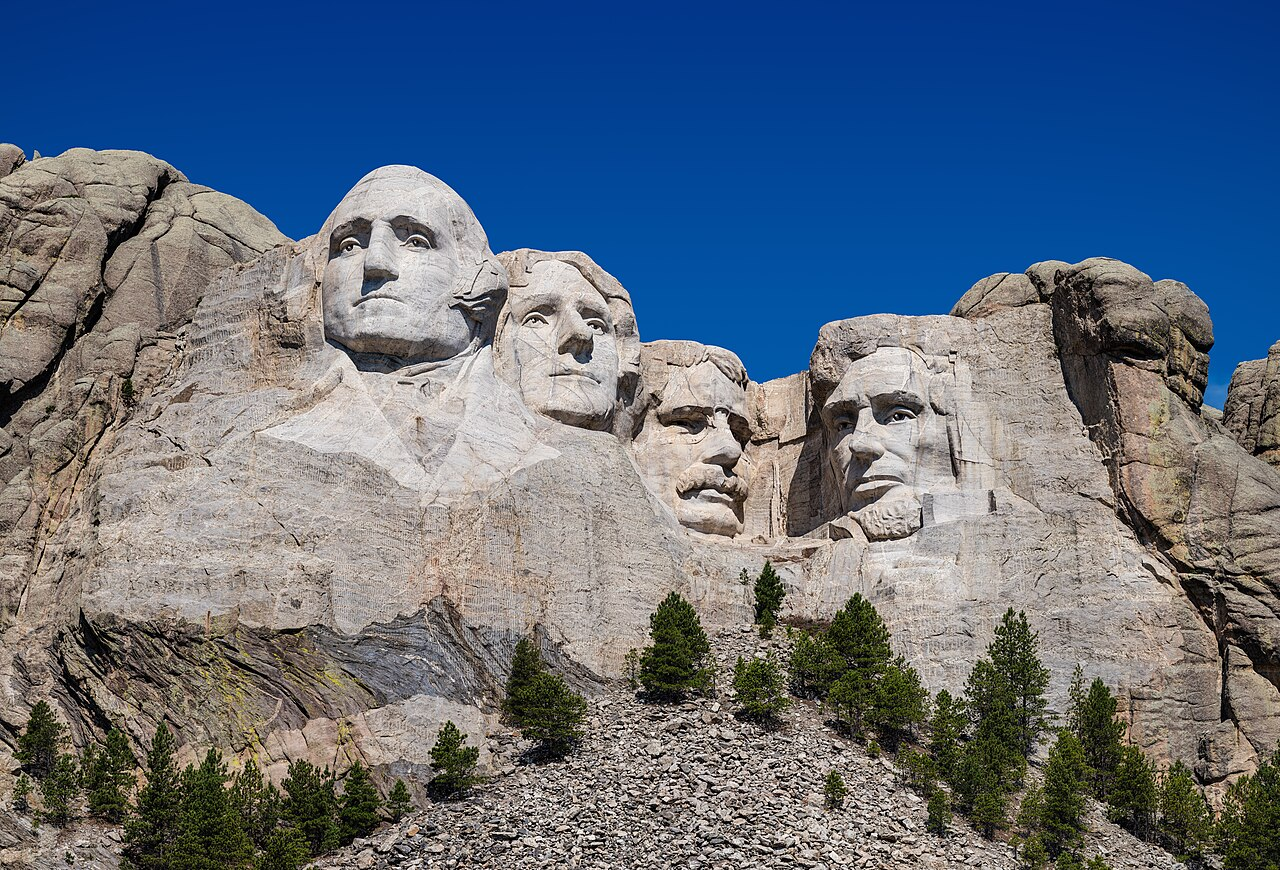
\includegraphics[width=7cm]{rushmore.jpg}};
        \foreach \x/\y/\n in {2.2/4.3/1, 3.1/3.95/2, 4.0/3.3/3, 4.95/3.4/4}
          \node[circle, fill=oldred, text=white, font=\small\bfseries, inner sep=0pt, minimum size=0.5cm] at (\x,\y) {\n};
      \end{tikzpicture}
      \credit{Photo: Thomas Wolf, www.foto-tw.de, CC BY-SA 3.0}
    \end{column}
    \begin{column}{0.42\textwidth}
      One point per president.\\[1em]
      \uncover<2>{%
      \opt{1}{George Washington}\\[0.5em]
      \opt{2}{Thomas Jefferson}\\[0.5em]
      \opt{3}{Theodore Roosevelt}\\[0.5em]
      \opt{4}{Abraham Lincoln}}
    \end{column}
  \end{columns}
\end{frame}

\begin{frame}{True or false?}
  \centering
  {\Large ``Mount Rushmore is a national park.''}\\[0.9em]
  \uncover<2>{%
  {\Large\alert{\textbf{False.}} It is a National \alert{Memorial}.}\\[1em]
  \begin{minipage}{0.5\textwidth}
    \begin{itemize}\setlength{\itemsep}{0.55em}
      \item Built 1927 to 1941
      \item Each head: 18 m tall
      \item Carved into the Black Hills
      \item Sacred land of the Lakota
    \end{itemize}
  \end{minipage}}
\end{frame}

% ===================== Round 7 =====================
\section{Round 7}
\whereis{Round 7}{denali2.jpg}{Photo: Gregory ``Slobirdr'' Smith, CC BY-SA 2.0}{usmap.png}{1280}
  {\hitdot{150}{650}{A}\mapdot{425}{355}{B}\mapdot{150}{60}{C}\mapdot{430}{750}{D}}
  {\alert{\textbf{A: Alaska}}\\[0.2em]{\normalsize Denali National Park}}

\begin{frame}{Denali}
  \begin{columns}[c]
    \begin{column}{0.52\textwidth}
      \begin{itemize}\setlength{\itemsep}{0.9em}
        \item North America's \alert{highest} mountain
        \item 6,190 m
        \item Gro\ss glockner: 3,798 m
        \item Name fight: Denali or Mount McKinley?
      \end{itemize}
    \end{column}
    \begin{column}{0.42\textwidth}
      \centering
      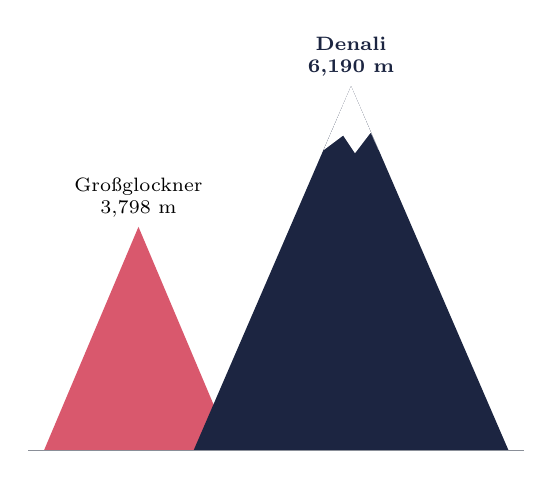
\begin{tikzpicture}[y=0.00075cm, x=1cm]   % 1 unit = 1 m
        \fill[austria!70] (0,0) -- (1.2,3798) -- (2.4,0) -- cycle;
        \fill[navy] (1.9,0) -- (3.9,6190) -- (5.9,0) -- cycle;
        \fill[white] (3.9,6190) -- (3.55,5100) -- (3.8,5350) -- (3.95,5050) -- (4.15,5400) -- (4.25,5100) -- cycle;
        \draw[muted] (-0.2,0) -- (6.1,0);
        \node[font=\scriptsize, align=center, above] at (1.2,3798) {Gro\ss glockner\\3,798 m};
        \node[font=\scriptsize\bfseries, align=center, above, text=navy] at (3.9,6190) {Denali\\6,190 m};
      \end{tikzpicture}
    \end{column}
  \end{columns}
\end{frame}

% ===================== Final round =====================
\section{Final Round: Bear Country}
\whereis{Final round}{brooks.jpg}{Photo: NPS / Michael Fitz, public domain}{alaska.png}{900}
  {\mapdot{450}{90}{A}\mapdot{450}{235}{B}\hitdot{410}{435}{C}\mapdot{735}{500}{D}}
  {\alert{\textbf{C: Katmai National Park}}\\[0.3em]{\normalsize About 2,200 brown bears\\More bears than people}}

\begin{frame}{Guess: you meet a bear}
  \centering
  A bear attacks you. \alert{Play dead} or \alert{fight back}?\\[0.6em]
  \begin{columns}[T]
    \begin{column}{0.4\textwidth}
      \centering
      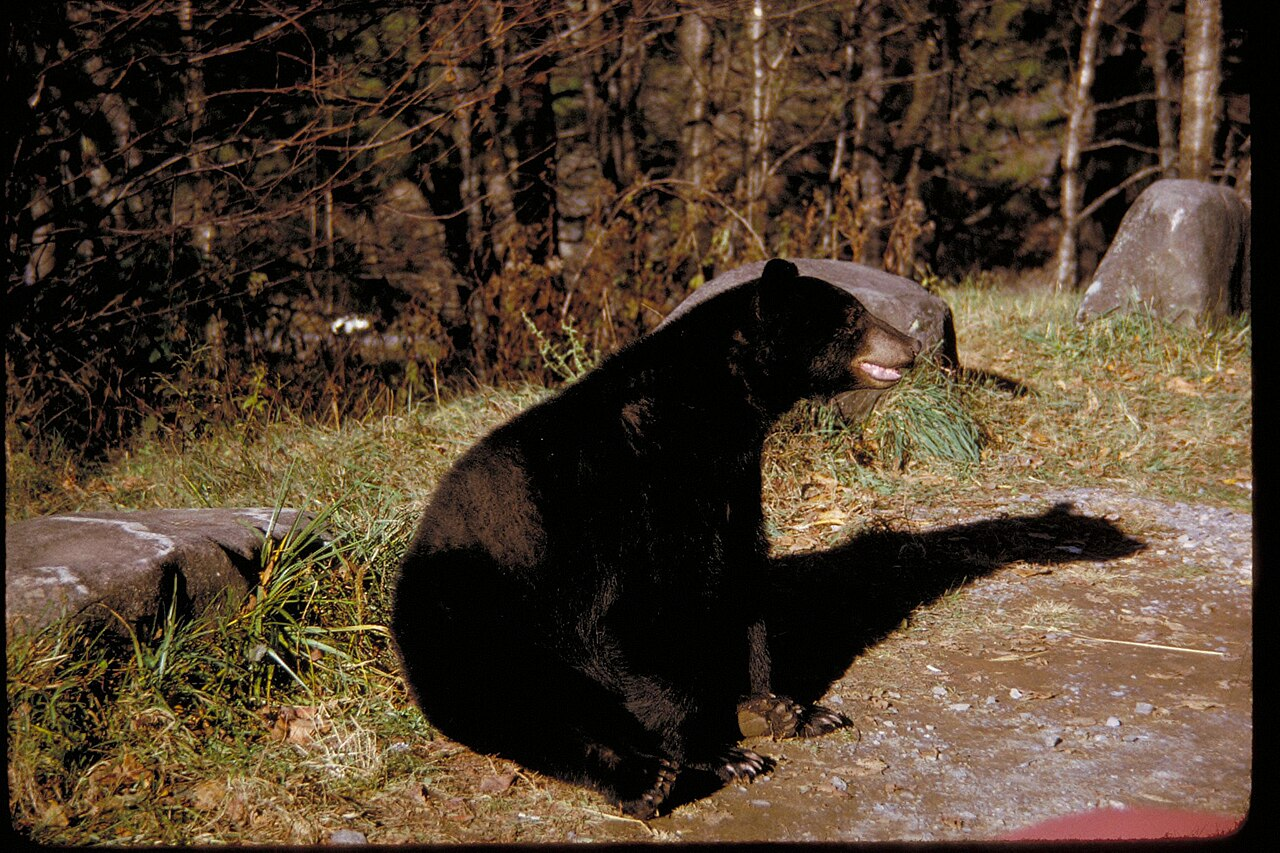
\includegraphics[height=3cm]{blackbear.jpg}\\[0.3em]
      {\bfseries\color{navy} Black bear}\\[0.2em]
      \uncover<2>{\alert{\textbf{Fight back}}}
    \end{column}
    \begin{column}{0.4\textwidth}
      \centering
      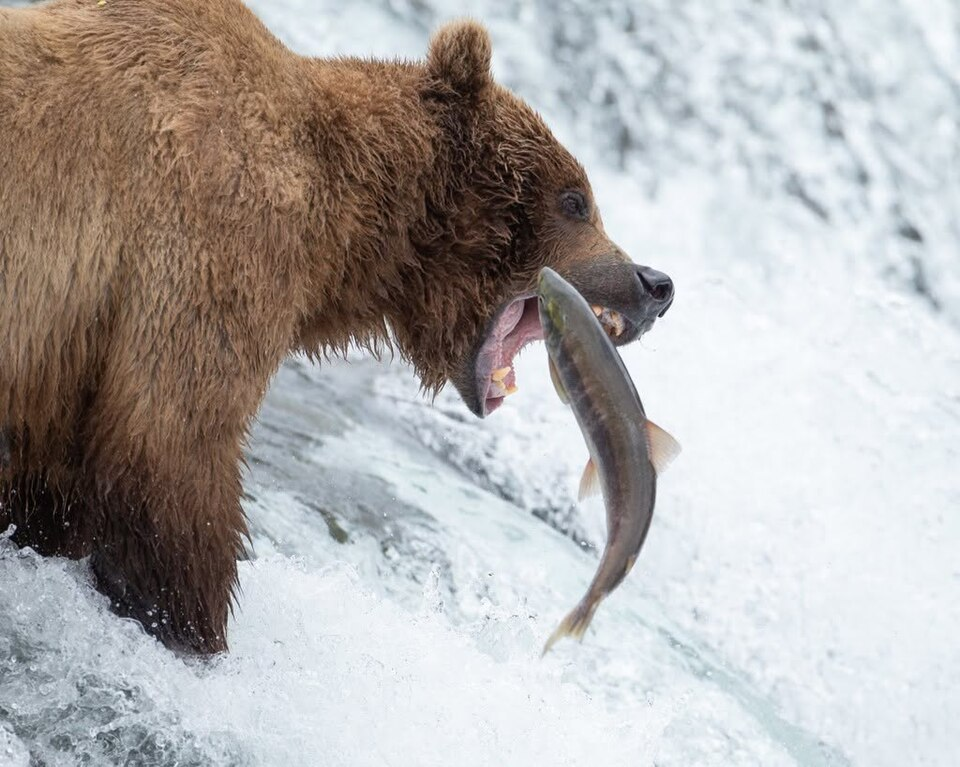
\includegraphics[height=3cm]{brooks2.jpg}\\[0.3em]
      {\bfseries\color{navy} Brown bear (grizzly)}\\[0.2em]
      \uncover<2>{\alert{\textbf{Play dead}}}
    \end{column}
  \end{columns}
  \vspace{0.7em}
  \uncover<2>{\emph{``If it's black, fight back. If it's brown, lie down.''}}
  \source{Source: National Park Service, ``Staying Safe Around Bears''. Photos: NPS; Peter Pearsall, public domain.}
\end{frame}

\begin{frame}{Meet Timothy}
  \begin{columns}[c]
    \begin{column}{0.5\textwidth}
      \begin{itemize}\setlength{\itemsep}{0.8em}
        \item Failed actor from New York
        \item \alert{13 summers} with wild grizzlies
        \item No gun, no bear spray
        \item Gave the bears names
        \item ``Mr.\ Chocolate'', ``Aunt Melissa''
      \end{itemize}
    \end{column}
    \begin{column}{0.44\textwidth}
      \centering
      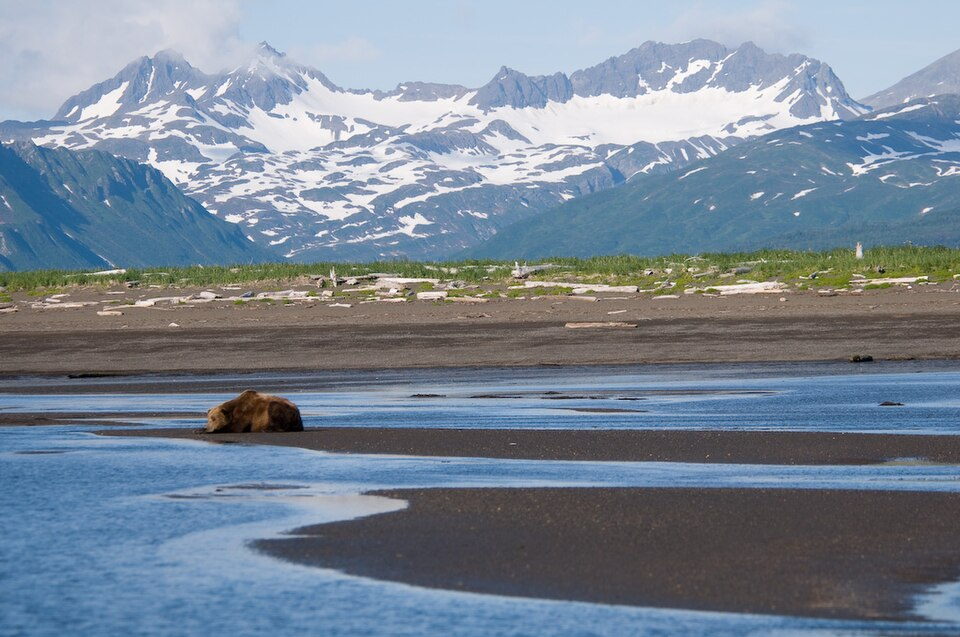
\includegraphics[width=\linewidth]{hallo.jpg}
      \credit{Hallo Bay, Katmai, where Timothy Treadwell camped. Photo: Marshmallow, CC BY 2.0}
    \end{column}
  \end{columns}
\end{frame}

\begin{thinkframe}
  {\color{oldred}\textbf{Think}}\\[0.8em]
  How does this story end?
\end{thinkframe}

\begin{frame}{October 2003}
  \begin{itemize}\setlength{\itemsep}{0.9em}
    \item Treadwell and girlfriend Amie Huguenard
    \item \alert{Killed by a bear} at camp
    \item The camera recorded sound only
    \item First bear deaths in Katmai's history
    \item 2005 film: \emph{Grizzly Man}
      (\href{https://www.youtube.com/results?search_query=Grizzly+Man+2005+official+trailer}{trailer})
  \end{itemize}
  \source{Sources: National Park Service; Alaska State Troopers (2003).}
\end{frame}

\begin{frame}{Hero or fool?}
  \centering
  \vspace{0.2cm}
  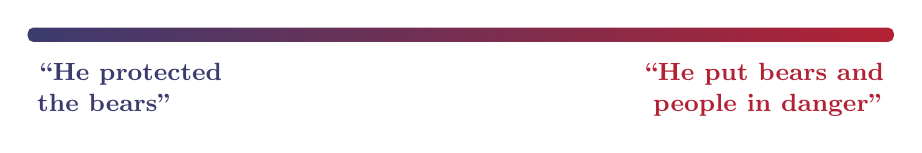
\begin{tikzpicture}
    \shade[left color=oldblue, right color=oldred, rounded corners=2pt] (0,0) rectangle (11,0.18);
    \node[anchor=north west, font=\small\bfseries, text=oldblue, align=left] at (0,-0.15) {``He protected\\the bears''};
    \node[anchor=north east, font=\small\bfseries, text=oldred, align=right] at (11,-0.15) {``He put bears and\\people in danger''};
  \end{tikzpicture}

  \vspace{0.6em}
  Stand where you agree. Tell your neighbour why.

  \vspace{0.8em}
  \begin{minipage}{0.72\textwidth}
    \begin{itemize}\setlength{\itemsep}{0.5em}
      \item \textbf{Supporters:} he taught thousands of schoolchildren
      \item \textbf{Critics:} bears lost their fear of people
      \item Rangers shot two bears afterwards
    \end{itemize}
  \end{minipage}
\end{frame}

\begin{frame}{Final scores}
  \begin{columns}[c]
    \begin{column}{0.5\textwidth}
      \begin{itemize}\setlength{\itemsep}{0.9em}
        \item Count your points
        \item Winning team: \alert{head rangers}
        \item Last question: which park would \alert{you} visit?
      \end{itemize}
    \end{column}
    \begin{column}{0.44\textwidth}
      \centering
      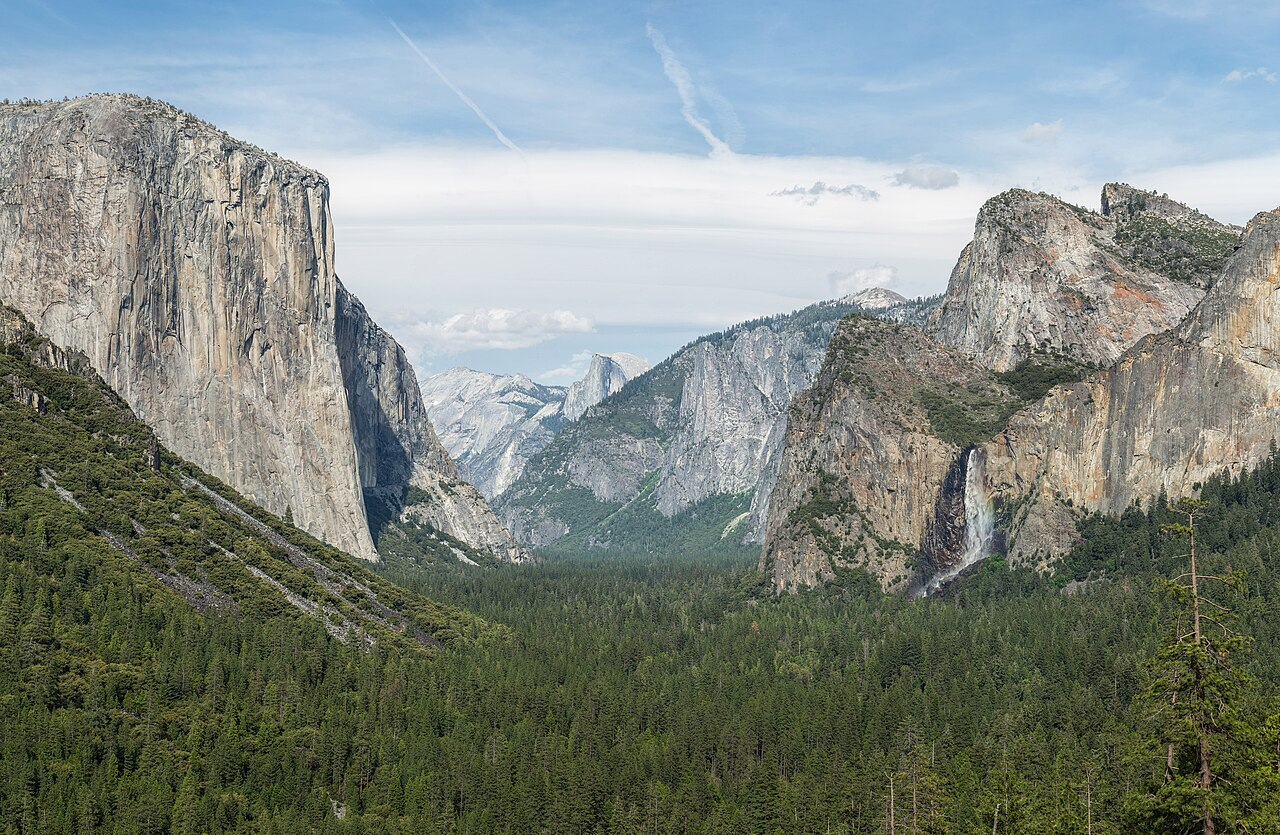
\includegraphics[width=\linewidth]{tunnelview.jpg}
      \credit{Yosemite Valley. Photo: Diliff, CC BY-SA 3.0}
    \end{column}
  \end{columns}
\end{frame}

\end{document}
